% ========================================================================================
%	Question 1
% ========================================================================================

\section{Introduction}

\subsection{The Team}
\begin{itemize}
    \item \textbf{Mikele Finn} - Team Lead - Business Administration major with managerial experience. Team lead and main spokesperson. Possibly the pilot?
    \item \textbf{Robert Edman} - Elder Statesman -- Lots of experience with problem solving and mechanical expertise.
    \item \textbf{Miranda Larson} - First Year <blank> major - Building and programming as well as design.
    \item \textbf{Kenneth Cloud} - Carpentry Major - With a background in programming and computer knowledge, our primary arduino guru.
    \item \textbf{Don Finn}
\end{itemize}


\subsection{Drone Design Philosophy}

Our design philosophy is one of flexibility. We would like our drone to be as flexible and versatile as possible, within the specifications of this kit. As a large, heavy drone, this machine lacks the maneuverability of traditional racing drones. What it lacks in maneuverability, it makes up for in power, longevity, and hauling power. We plan to include a full instrument package, sampling apparatus, and imaging array (either one or two full video cameras).

The instrument package will contain proximity and distance sensors, gyroscope, hall effect sensors, temperature, humidity, and <Add More>.

Our sampling apparatus will be designed to retrieve samples of both solids and liquids. A vial, a scoop, and possibly a grabbing arm.

\section{Progress}

\subsection{Blue Heron}

Two students have practiced flying the Blue Heron, though much work remains to be done in this area. We still have not selected our pilot. The plan will be for everyone to practice as much as possible doing some precision flying of the Blue Heron and whoever is most comfortable with it, will graduate to <Need Name>. All students are expected to be passably competent so we have backups in case of illness on the day of the event.

\subsection{Flame Wheel}

\begin{figure}[!htbp]
\centering 
        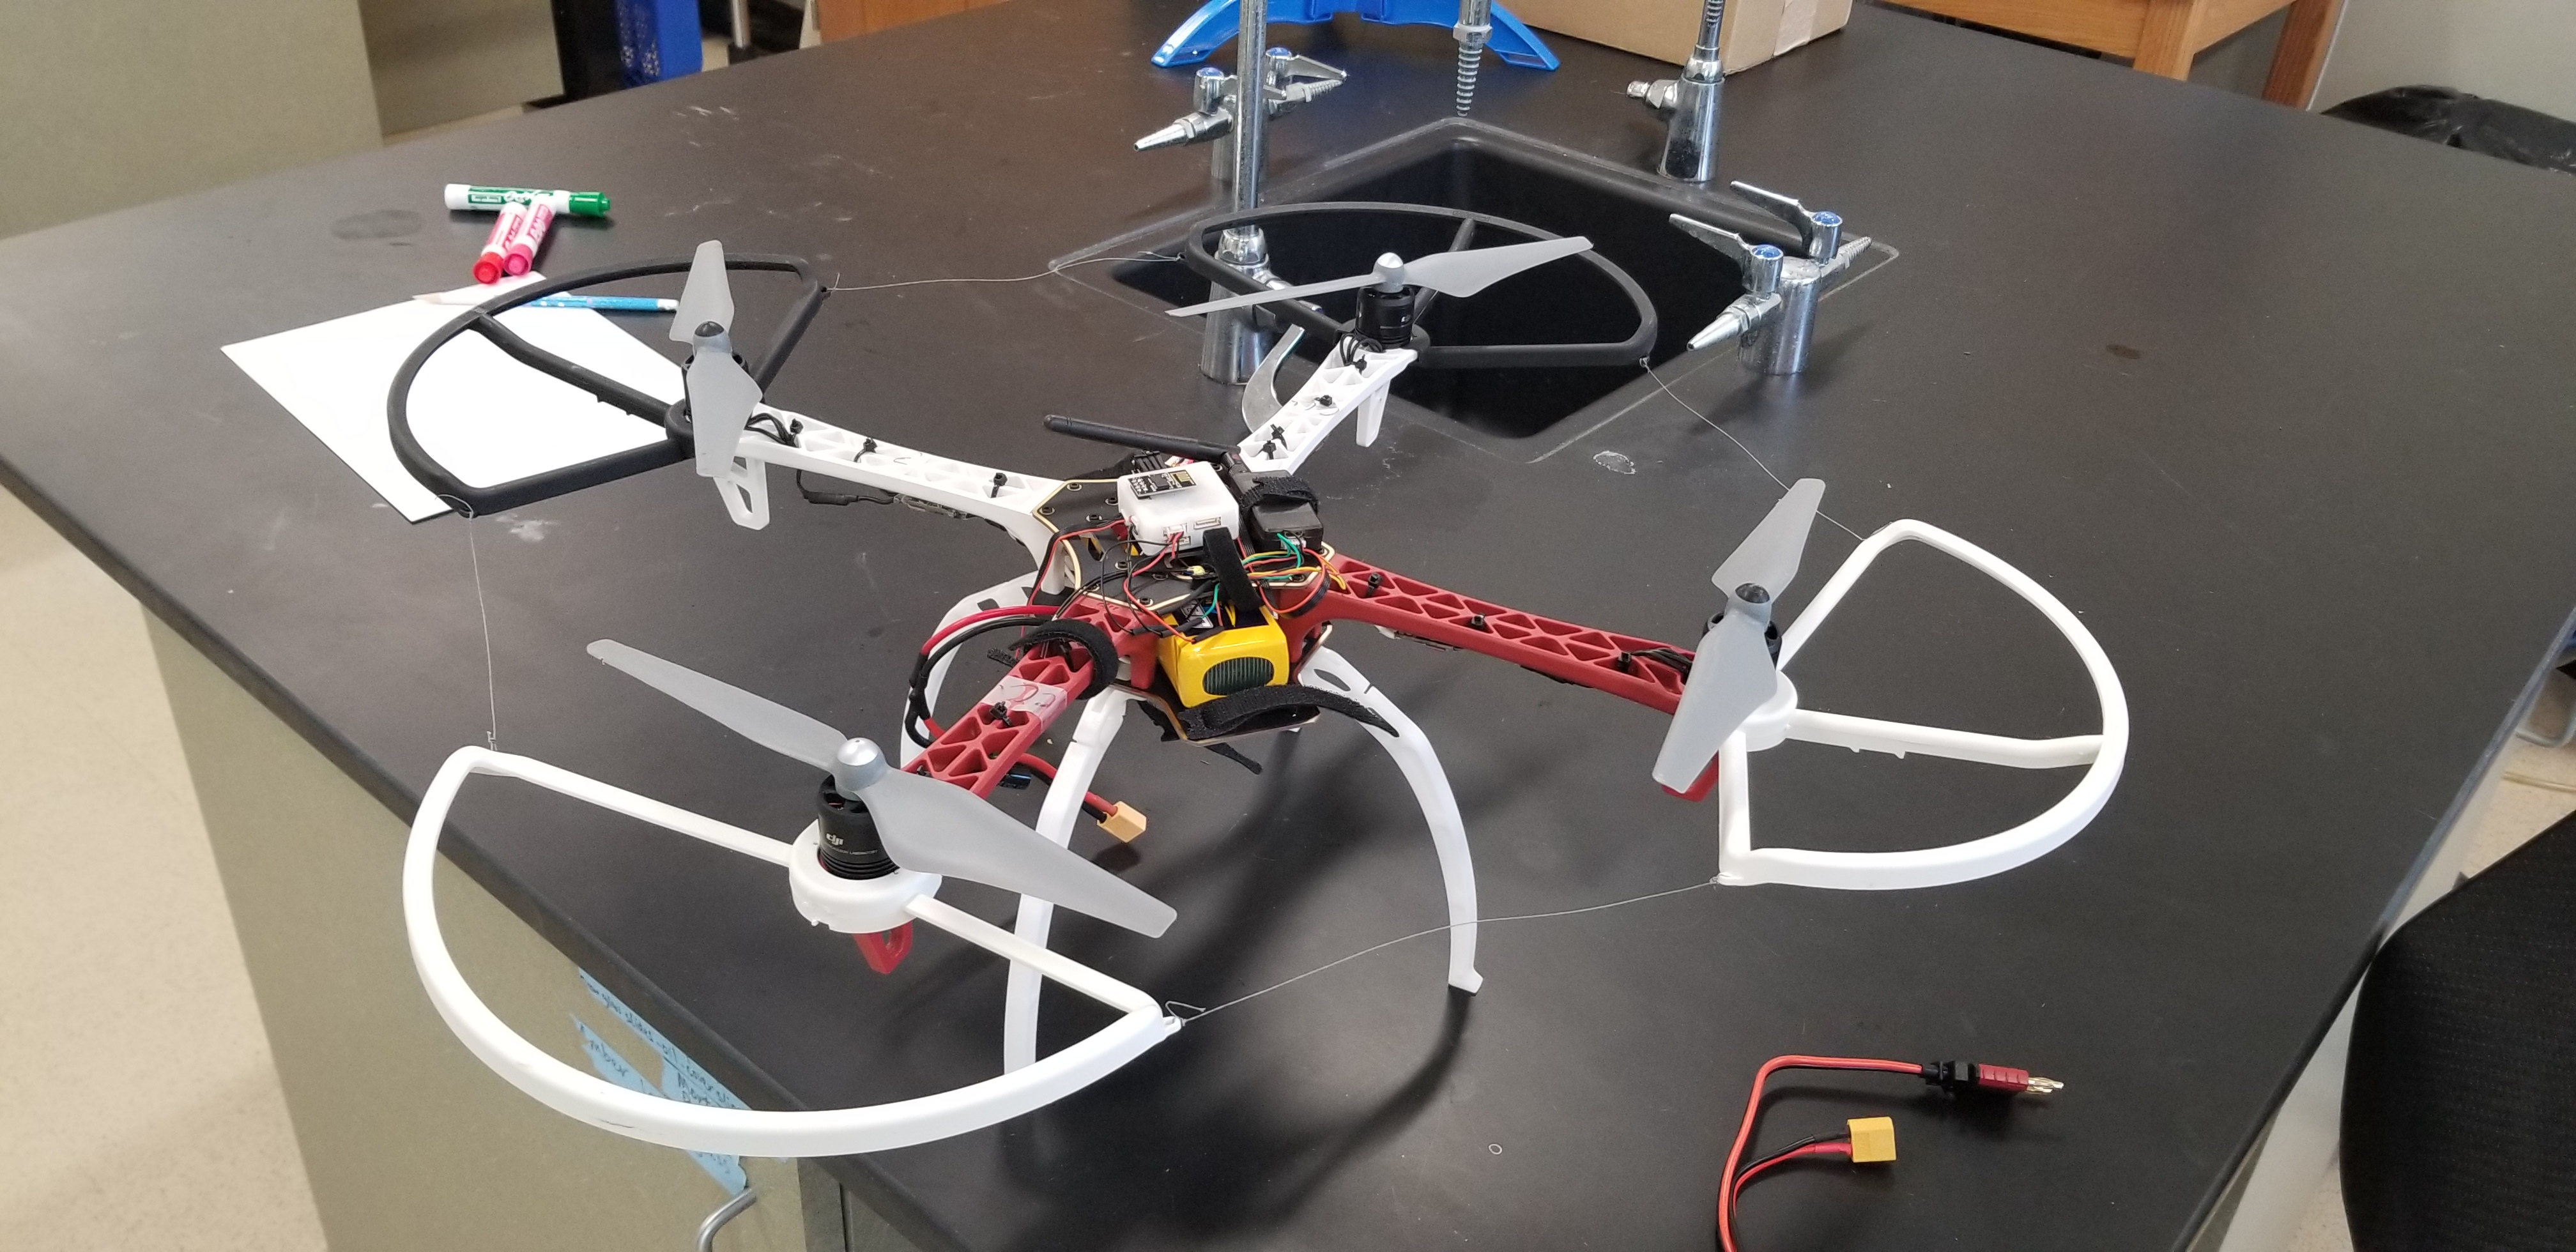
\includegraphics[width=0.5\textwidth]{figs/flamewheel1.jpg}
\caption[Completed airframe]{Completed airframe}
\label{fig:airframe} 
\end{figure}

The Flame Wheel basic airframe is complete, calibrated, tuned, and has made its first few flights, from simple hovers to moving about a large room (Figure: ~\ref{fig:airframe}). We have not set up a practice course yet, but expect to soon.

The build went fairly smoothly. The frame went together without incident. After the main assembly of the airframe, programming and calibration were completed successfully, followed by an attempted first hover. This resulted in an immediate and spectacular crash. After some diagnosis and one more crash (which resulted in damage to one of the propeller guards), it was determined that the ESCs were simply connected to the incorrect ports on the flight controller. Finally, a proper flight test was conducted in which the drone was secured with shock cables to our work bench.

\begin{figure}[!htbp]
\centering 
        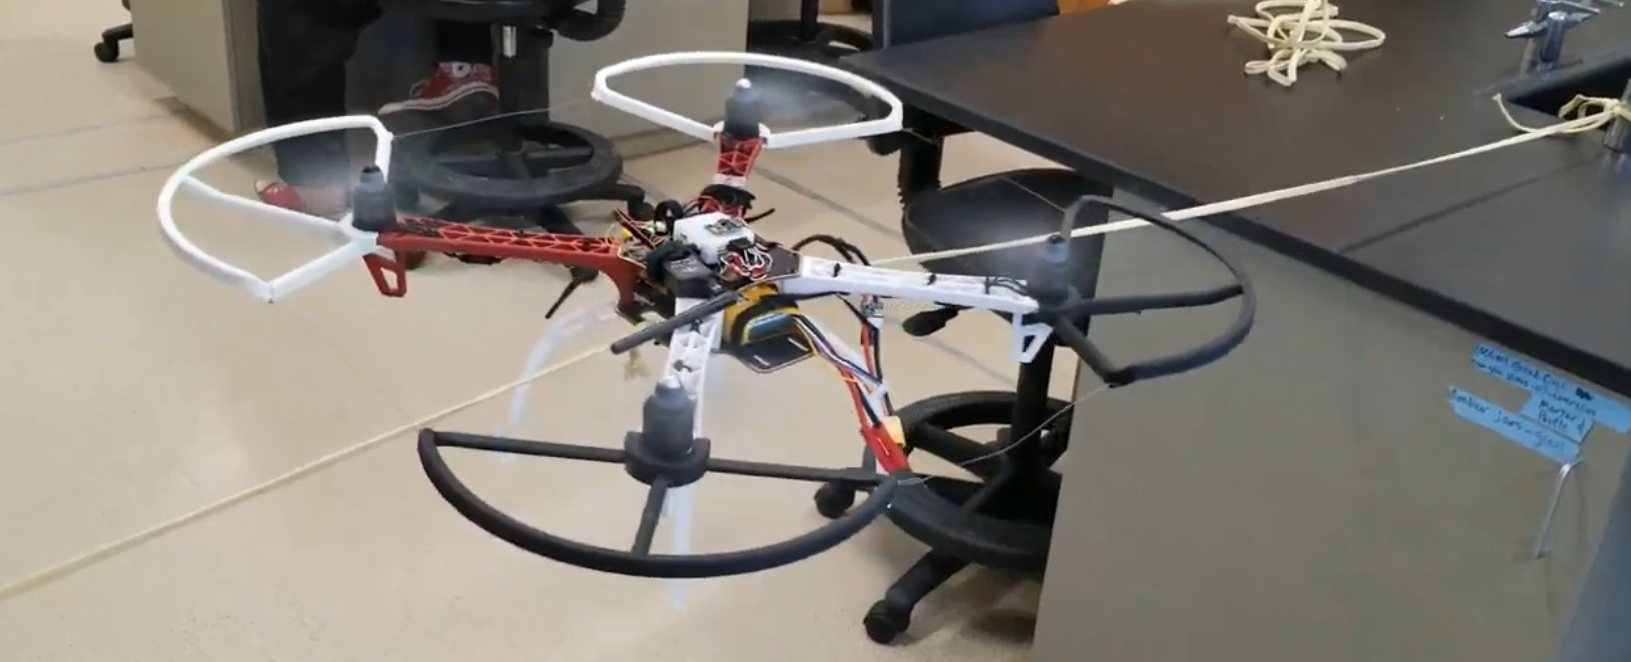
\includegraphics[width=0.5\textwidth]{figs/tune.png}
\caption[Tuning the drone]{Tuning the drone}
\label{fig:tuning} 
\end{figure}

This method of securing the drone to test the PID tuning and ended up being considerably safer and allowed us to be much more confident before attempting a real flight (Figure: ~\ref{fig:tuning}).

As for instrumentation, we are still in the planning and implementation stage. Sensor suite is still a wishlist, and ordering of parts will take place soon.

\section{Progress and Plans for the Challenge}

\begin{figure}[!htbp]
\centering 
        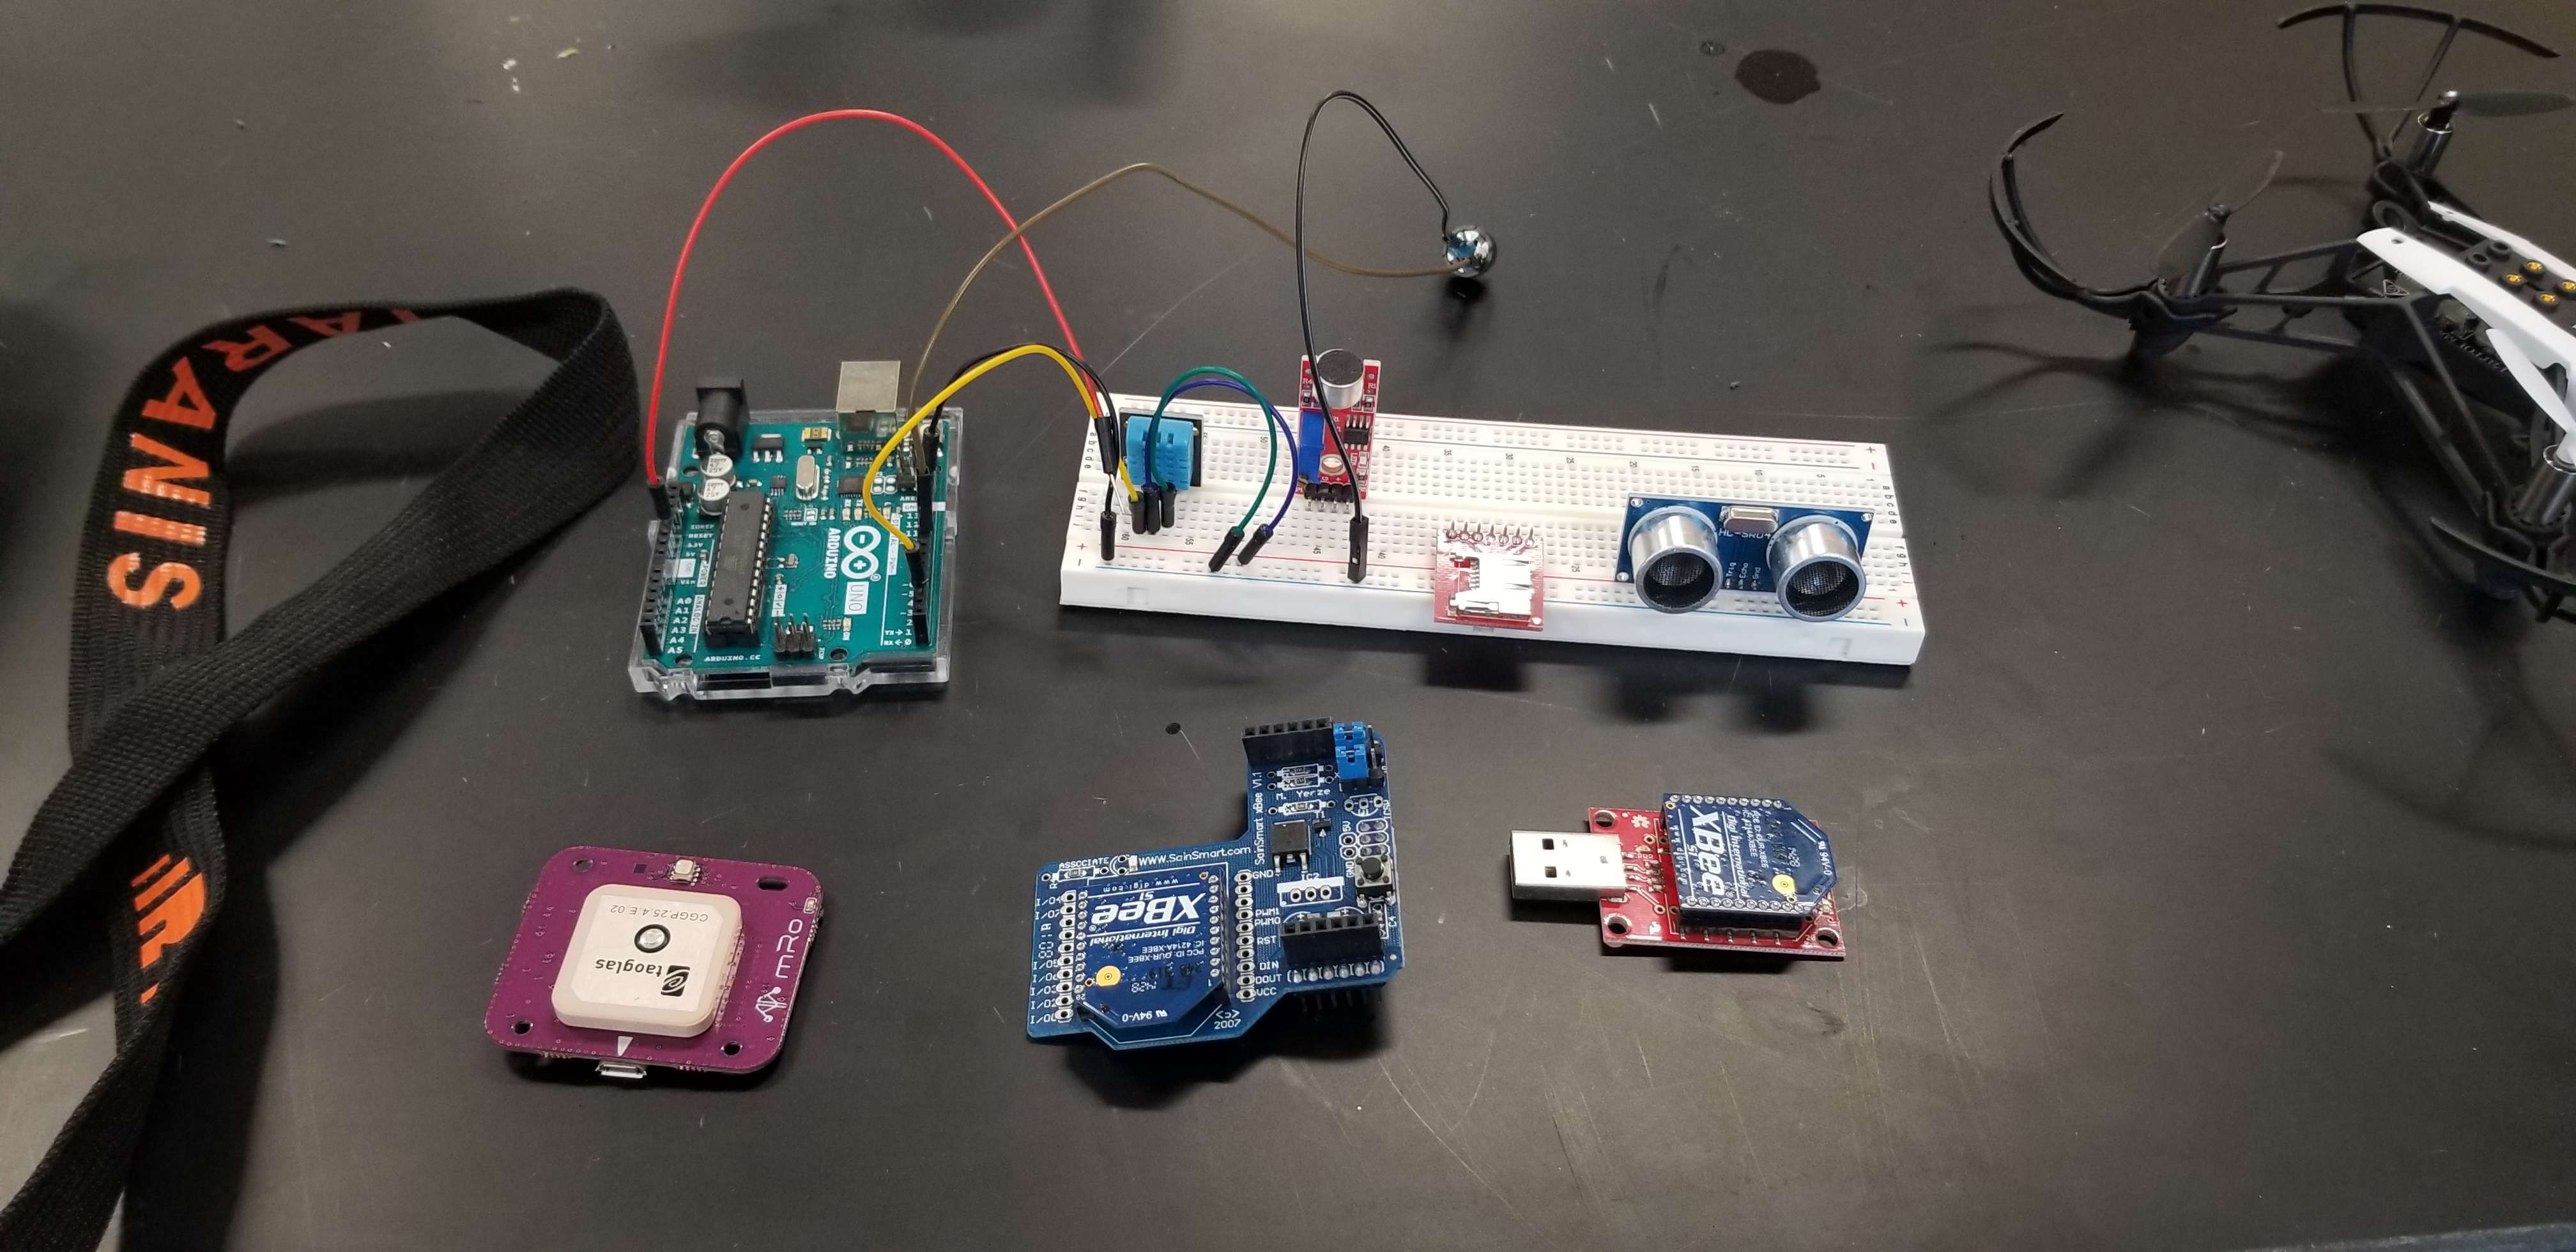
\includegraphics[width=0.5\textwidth]{figs/electronics.jpg}
\caption[Sensor suite and XBee radio]{Sensor suite and XBee radio}
\label{fig:electronics} 
\end{figure}

We have built a few proof-of-concept sensor packages and written code for them. The next step is to order all of the sensors and actuators that we need and to integrate the code for each individual sensor, motor, and communication device. (Figure: ~\ref{fig:electronics})

We will be placing an order for our final sensor suite very soon, and have recruited a student with programming experience which will help to speed up progress on this front.

The plan is to use XBees to transmit all data back to the home base computer in real time.

We would like to, in the end, modularize our instrumentation. If, on competition day, we can swap out instrumentation modules on the fly, we will have a lot of flexibility in handling the sorts of challenges which the course might present.

\section{Plans for Challenge: Flight Day Operations}

We plan to have two or three operators during the flight. To prepare for the flight, we will observe the course and plan a route through it to determine where we want to stop and investigate. The actual operation of the drone will consist of two or three stations. These three stations are:

\begin{itemize}
\item \textbf{Pilot:} Holds the transmitter and pilots the drone. If we have visual on the course, from where the pilot is stationed, they can do some reckoning that way, but there will be a few cameras transmitting video back to a tablet in real time for fine maneuvering.
\item \textbf{Sensors:} Another operator will have access to video feeds and readouts transmitted via XBee from the drone’s instrument package. This operator’s job will be to record measurements from sensors and keep track of points of interest throughout the course.
\item \textbf{Engineering:} A third operator (it is possible that Engineer and Sensors will be merged into one station) will be in charge of activating any actuators that are built into the drone. This will include various sampling mechanisms (scoops and such) that need to be controlled separately from piloting.
\end{itemize}

\section{Organizational Chart}

\# TODO

\section{Budget and Parts List}

\# TODO

\section{Schedule}

\# TODO

\section{References}

\# TODO

\section{Appendices}

\# TODO

